The enormous benefits that CMOS technology scaling has brought have come along with an increase in variability. Not only \gls{TZV}, existing after fabrication, but \gls{TDV} effects, like aging, are becoming more relevant. Some examples of \gls{TDV} phenomena are \gls{BTI} or \gls{HCD}. These phenomena show a stochastic nature, which makes them much harder to model. To address this issue, stochastic defect-centric models~\cite{grasserParadigmShiftUnderstanding2011, reisingerUnderstandingModelingAC2011, kaczerDefectcentricPerspectiveDevice2015} such as the Probabilistic Defect Occupancy (PDO) model \cite{martin-martinezProbabilisticDefectOccupancy2011} are used. Parameter extraction for these models requires massive device characterization so that statistically significant information is obtained \cite{saraza-canflancaDeterminationTimeConstant2022}. Once these parameters are obtained, the model can be integrated in a simulation tool, and circuit reliability predictions made to prevent the impact of aging on the final design \cite{amrouchMLRescueReliability2023,klemmeMachineLearningCircuit2021,klemmeScalableMachineLearning2022a,klemmeEfficientLearningStrategies2022}. Accuracy is critical, as overcompensation leads to unnecessary performance loss and undercompensation to early circuit failure. Specifically, in digital circuits, aging generally results in a longer propagation delay for logic gates, ultimately leading to potential timing violations.

The aging of each transistor inside a logic gate is highly dependent on its biasing (ON/OFF time) \cite{vansantenNewWorstcaseTiming2019, santana-andreoImpactBTIHCI2022}. Given how each transistor's bias depends on the input values of the logic gate, a logic gate can go through different degradation scenarios depending on the inputs it has during its lifetime. Consequently, to fully understand how aging affects digital circuits, performing characterization at the device level is not enough. However, characterization at the circuit level is still a nascent topic in the reliability community \cite{santana-andreoCharacterizingAgingDegradation2022, saraza-canflancaSmartSRAMCellArray2022}, and no large-scale characterization that takes into account the dependency of aging on gate inputs has been made before this work. Consequently, the first pillar of this thesis is \textbf{Characterization}. To address this issue, a chip named ATIUM has been designed capable of measuring the aging of each individual gate. 

On the modeling side, defect-centric models can deliver the degradation of a transistor given a certain biasing. Nevertheless, their application to large-scale digital circuits operating under realistic workloads over typical system lifetimes is limited because of the computational complexity of these models. To make the application of aging models in that context feasible, a useful technique is to compress the transistor workloads \cite{vansantenDesigningGuardbandsInstantaneous2016,AtomisticPseudoRodopoulos2014, duchAnalysisFunctionalErrors2020}. However, existing compression techniques have shortcomings that result in inaccurate degradation values. Two new compression techniques are proposed to compress workloads with minimal accuracy loss (1.31\% and 2.31\% average error respectively, compared to $>$ 70\% average error for the approaches found in the literature) while achieving execution speeds sufficient for large digital circuits (1,151 and 146 seconds, respectively, compared to 10 hours for the reference uncompressed workload, for a benchmark circuit with 3100 transistors). Through these techniques, accurate degradation predictions can be performed which enable designers to mitigate aging at design time. Accordingly, the second pillar of this thesis is \textbf{Mitigation}.

Finally, the third and last pillar is \textbf{Exploitation}. \gls{TZV} can be exploited in the field of hardware security to create \glspl{PUF}. \glspl{PUF} exploit the intrinsic variability of circuits to create unique fingerprints, through which each circuit instance can be uniquely identified taking advantage of already existing circuitry, i.e., at a low cost. Specifically, the popular \gls{SRAM} \glspl{PUF} \cite{saraza-canflancaImprovingReliabilitySRAMbased2021, santana-andreoDRVbasedBitSelection2022, santana-andreoReliabilityImprovementSRAM2024a} employ the power-up value of \gls{SRAM} cells, which is heavily dependent on variability. However, \glspl{PUF} have a critical limitation: their reliability. A \gls{PUF} must always provide the same response. Being reliant on small \gls{TZV} differences, they are very sensitive to changes due to temperature, voltage, or \gls{TDV} phenomena. \glspl{ECC} are employed to solve this, however, these \glspl{ECC} come at a high implementation cost in terms of area, going against one of the selling points of \glspl{PUF}: their low cost of implementation. In this work, the understanding of \gls{TDV} provides a method for selecting the most stable cells on an \gls{SRAM} \gls{PUF} and significantly reducing the required \gls{ECC}. In the next subsections, the contributions in each of these three pillars are described in more detail. 

\begin{figure*}
    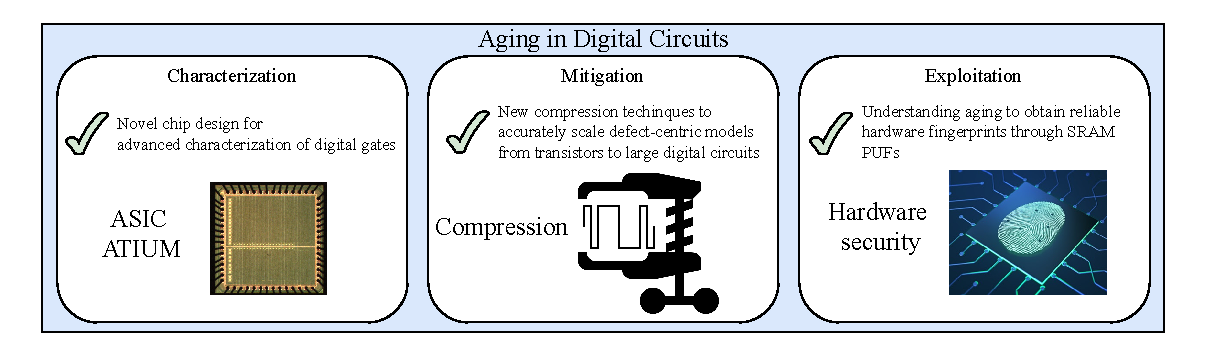
\includegraphics[width=\textwidth,trim={6mm 2mm 6mm 3mm},clip]{images/DATE.pdf}
    \caption{Summary of the three pillars of this thesis: Characterization, Mitigation and Exploitation.}
    \label{fig:PDO_Intro}
\end{figure*}

\section{Characterization}

ATIUM is a chip designed in a 65-nm CMOS technology for the characterization of aging effects on digital cells, specifically logic gates. The chip uses accelerated aging techniques to measure the degradation caused by aging. Thus, a \gls{CUT} is characterized before (when it is fresh) and after accelerated aging is applied, i.e. after a stress (excess supply voltage and/or temperature) is applied. The goal is to determine the increased delay of the \gls{CUT} due to aging degradation. To measure the delay of a \gls{CUT}, the typical approach followed in the literature is to connect a number of \glspl{CUT} as a \gls{RO} \cite{kimSiliconOdometerOnchip2008, keaneArraybasedOdometerSystem2011, parkAllBTINPBTI2021, islamCalibrationFreeSynthesizableOdometer2022}. The sum of the delays of all the \glspl{CUT} determines the oscillating frequency. Accordingly, if the \gls{CUT} delay is affected by aging, we can extrapolate the degree of aging degradation the cell suffers by comparing the frequency of the \gls{RO} before the \gls{CUT} is stressed with the frequency of the \gls{RO} after the \gls{CUT} has been stressed. This measurement is performed on-chip through the use of ``aging odometers'', which give the degree of aging degradation as a digital output by comparing the \gls{RO} frequency to a reference frequency using a phase comparator \cite{kimSiliconOdometerOnchip2008, keaneArraybasedOdometerSystem2011, parkAllBTINPBTI2021, islamCalibrationFreeSynthesizableOdometer2022}. However, including multiple \glspl{CUT} in a \gls{RO} has the disadvantage of averaging out the stochasticity of \gls{TDV} and having only one input through which oscillations are possible. To address this, in ATIUM, a novel topology is employed. Instead of measuring a chain of \glspl{CUT}, a single \gls{CUT} is measured with the help of an auxiliary \gls{RO}. In this way, the supply, inputs and output of the \glspl{CUT} are independently controlled so that the \gls{CUT} can be placed under stress in isolation, in stand-by or be measured by one of its inputs. The \glspl{CUT} used are standard logic gates with 3 inputs, having different propagation delays associated with each input. Thanks to this setup, the \glspl{CUT} can be stressed under any combination of DC or AC voltages on the desired inputs, and then measured through any of its inputs, without losing stochastic information. This enables, for the first time, to measure the complex relationship between biasing and degradation predicted by simulated models and certify the importance of accurate aging simulation. In ATIUM, numerous \glspl{CUT} are included (1152 per chip, which can be stressed in parallel) to perform statistically relevant characterizations.


\section{Mitigation}

To evaluate the aging degradation of each digital gate, we employ our circuit-level aging simulator, CASE \cite{martin-lloretCASEReliabilitySimulation2017}. CASE works with a certain circuit netlist as input, simulates the circuit topology with the SPICE circuit simulator taking into account aging variability and returns the aging-induced degradation per transistor and the circuit's aged performances. A custom script is employed to build a reliability framework to extend CASE from small circuits like individual cells to large scale circuits with thousands of cells. After a thorough exploration of the compression techniques found in the literature, we have successfully introduced two novel approaches that surpass existing methods in terms of speed and accuracy. The accuracy of each compression method is evaluated wholistically, i.e., with aging-aware circuit delay estimations that can take into account the stochasticity of \gls{TDV}. To mitigate the effect of aging in digital circuits, a guardband (i.e., a timing slack on top of circuit delay) is typically used. When no stochasticity information is available, a pessimistic, worst-case degradation is uniformly applied to all transistors. Meanwhile, by building accurate \gls{TDV}-aware cell libraries, the required timing guardband is significantly reduced \cite{vansantenModelingMitigatingTimeDependent2019}. The computational challenge of building workload-specific \gls{TDV}-aware cell libraries can be solved through the use of ML techniques \cite{klemmeEfficientLearningStrategies2022, klemmeMachineLearningCircuit2021, klemmeScalableMachineLearning2022a}. By employing our high-performing compression techniques, we are able to expand on these works, bringing the stochastic predictions of defect-centric models to the standard digital design flow accurately. 



\section{Exploitation}
The work in \gls{SRAM} \glspl{PUF} \cite{saraza-canflancaImprovingReliabilitySRAMbased2021, santana-andreoDRVbasedBitSelection2022, santana-andreoReliabilityImprovementSRAM2024a} provides two main contributions. First, by performing an in-depth exploration of characterization results of \gls{SRAM} cells after accelerated aging, it has been shown that due to the stochastic nature of reliability phenomena in scaled CMOS technologies, different cells will suffer different degradation even under the same stress conditions. Traditionally, only \gls{BTI} is considered to model degradation in \gls{SRAM} \glspl{PUF}. However, it was also shown how \gls{NC-HCD} also plays an important role. Second, a technique based on measuring the \gls{DRV} of each \gls{SRAM} before stress is proposed. This technique quantifies the skew of each cell to power up to one state or another, and is able to predict the robustness of each cell to \gls{TDV} phenomena. The higher the \gls{DRV}, the higher the skew, with each cell having a certain \gls{DRV} (skew) to power-up to ``1'' or ``0''. By selecting those cells with a high \gls{DRV} value in one direction and a null \gls{DRV} value in the other, very reliable cells are employed, reducing considerably the overhead associated with \glspl{ECC}. This is proven by the extensive aforementioned characterization data. 